\section{Exploración y limpieza de datos}
Una vez seleccionados los conjuntos de datos, el siguiente paso consiste en conocerlos a fondo. La fase de exploración del ciclo CRISP-DM no es un trámite previo al modelado: es el momento en que las hipótesis del negocio se contrastan por primera vez contra la evidencia y, sobre todo, donde se identifican los problemas estructurales que de no resolverse contaminarían los resultados. En esta sección recorremos las cuatro fuentes que sostienen el proyecto. En cada una hacemos lo mismo: cargamos los datos sobre el cluster Spark, los exploramos para entender su comportamiento, valoramos su calidad y proponemos las transformaciones iniciales necesarias para llevarlos a un estado utilizable. Los gráficos que acompañan cada subsección no son ilustrativos: son el insumo principal sobre el cual se tomaron las decisiones de limpieza posteriores.

\subsection{Resultados Saber 11 (ICFES)}
El dataset Saber 11 es el corazón del proyecto. Es la fuente que contiene la variable que el Ministerio quiere mejorar y, a la vez, la fuente que más reto técnico impuso por su volumen. La base consolidada en HDFS alcanza los 7,109,704 registros y 51 columnas, donde cada fila corresponde a un estudiante que se inscribió a la prueba. Esto, en términos de Spark, se traduce en alrededor de 3.5 GB de información comprimida que el cluster lee y procesa en paralelo sobre sus cuatro workers.

\textbf{Lo primero que miramos: el puntaje.} La variable \texttt{PUNT\_GLOBAL} es la columna que define el éxito o fracaso de cualquier predicción posterior. Su distribución es muy informativa por sí sola.

\begin{figure}[H]
\centering
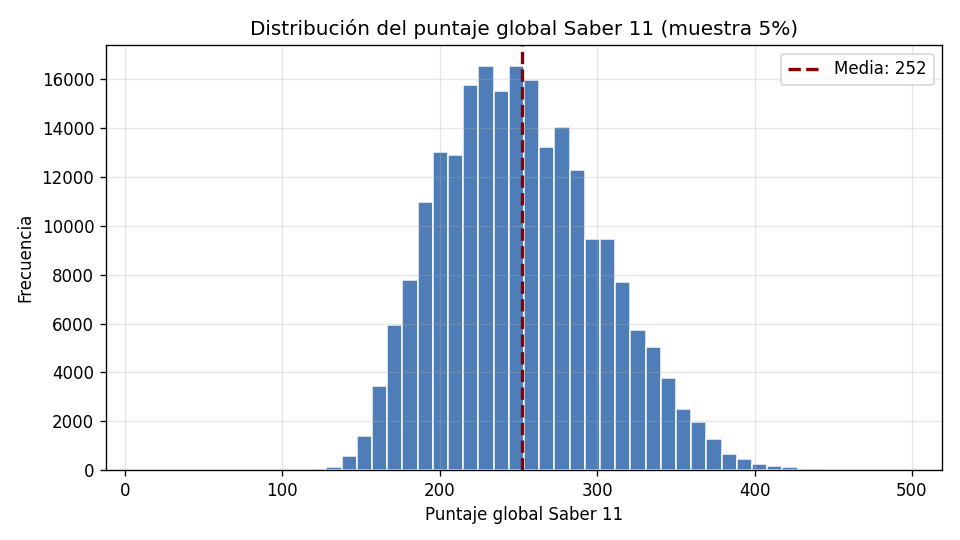
\includegraphics[width=0.85\textwidth]{figures/icfes_hist_punt_global.png}
\caption{Distribución del puntaje global Saber 11. La línea roja marca la media. La cola izquierda en cero corresponde a registros no presentados.}
\end{figure}

El histograma confirma lo que el promedio nacional sugiere: la mayoría de los estudiantes obtienen entre 200 y 300 puntos, con una media cercana a los 250 puntos, una desviación amplia y una cola larga hacia arriba. El detalle más importante de este gráfico, sin embargo, no es la forma de la curva sino la presencia de una concentración anómala en el extremo izquierdo: aproximadamente 2.6 millones de registros tienen puntaje nulo, lo que en términos prácticos significa que el estudiante no presentó la prueba o que el registro está incompleto. Esa observación, evidente al graficar, marcó la primera decisión de limpieza: cualquier modelo que prediga el puntaje debe entrenarse sobre los registros que efectivamente lo tienen.

\textbf{La geografía cuenta.} Al agregar los puntajes por departamento aparecen las primeras diferencias territoriales del análisis.

\begin{figure}[H]
\centering
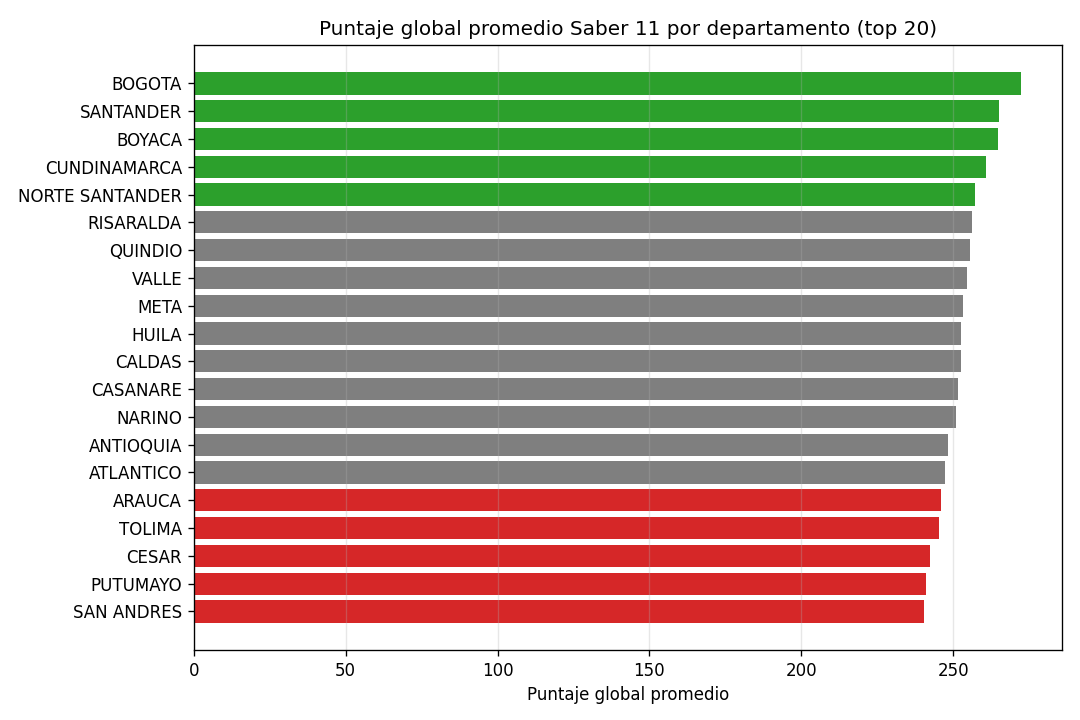
\includegraphics[width=0.9\textwidth]{figures/icfes_depto_top.png}
\caption{Puntaje global promedio por departamento (top 20, mínimo 1,000 estudiantes). Verde: los cinco mejores. Rojo: los cinco con menor puntaje del top 20.}
\end{figure}

El ranking muestra el patrón esperado: Bogotá, Santander, Boyacá y Antioquia concentran los puntajes más altos del país, mientras que departamentos como Chocó, Vichada y La Guajira aparecen en la parte baja. La diferencia entre los extremos supera los 30 puntos, lo que en escala Saber 11 es una brecha estructural enorme. Vale la pena anotar que la palabra "departamento" aparece escrita de distintas formas en los datos originales (con y sin tildes, en mayúscula, minúscula y mixto), lo que obligó a aplicar una normalización temprana: pasar todo a mayúsculas, remover acentos y descartar valores nulos en la geografía. Sin esa limpieza, Bogotá y BOGOTÁ habrían aparecido como dos territorios distintos en el mismo gráfico.

\textbf{Internet en el hogar: ¿hace diferencia?} La pregunta central del proyecto se puede empezar a responder con un solo cruce.

\begin{figure}[H]
\centering
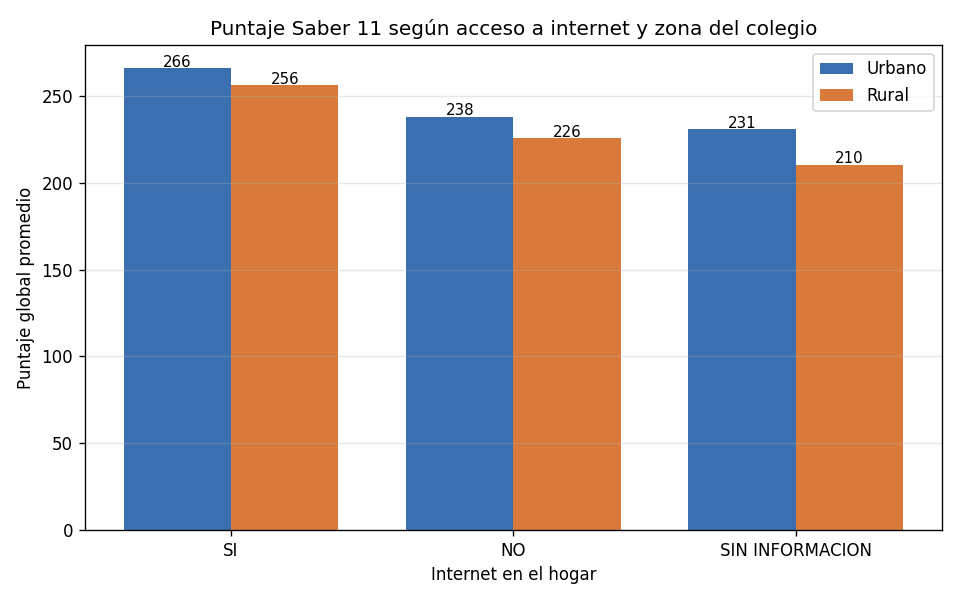
\includegraphics[width=0.85\textwidth]{figures/icfes_internet_zona.png}
\caption{Puntaje global promedio según acceso a internet en el hogar y zona del colegio.}
\end{figure}

El gráfico es contundente: tanto en zona urbana como en zona rural, los estudiantes con internet en el hogar obtienen un puntaje promedio claramente superior a los que no lo tienen. La brecha urbana ronda los 13 puntos, y la brecha rural es de magnitud similar, lo que sugiere que el efecto del acceso digital no es exclusivo de un tipo de territorio. Adicionalmente, la categoría \texttt{SIN INFORMACION} se comporta más parecido al grupo sin internet, lo que da una pista interesante: probablemente quienes no responden la pregunta también pertenecen a hogares vulnerables. Este es exactamente el tipo de observación que dispara una decisión de transformación: en lugar de descartar los nulos, conviene tratarlos como una categoría informativa propia, lo que después se hace explícito en la capa Silver.

\textbf{Calidad y volumen.} La exploración deja en evidencia varias cosas. La primera, ya mencionada, es que el 37\% de los registros no tiene puntaje global. La segunda es que variables como acceso a internet, computador y estrato familiar están mayoritariamente completas, lo que las habilita como features para los modelos. La tercera es que los puntajes por área (lectura, matemáticas, ciencias, sociales, inglés) llegan en formato de texto con coma decimal, lo que requiere un parseo cuidadoso. Estas observaciones se traducen en las transformaciones formales documentadas en la siguiente sección del documento, donde se especifica cada filtro y cada cast con su justificación.

\subsection{Internet Fijo (MinTIC)}
El dataset de Internet Fijo es la fuente de conectividad por excelencia del proyecto. Su grano es muy fino: cada fila representa un reporte trimestral de un proveedor en un municipio, desagregado por tecnología y segmento. La base consolidada en Spark tiene 2,795,052 registros y 12 columnas, lo que se traduce en aproximadamente 384 MB en HDFS. La pregunta principal a responder con este dataset es cómo ha evolucionado el servicio en el tiempo y cómo se distribuye geográficamente y tecnológicamente.

\textbf{La evolución temporal cuenta una historia clara.}

\begin{figure}[H]
\centering
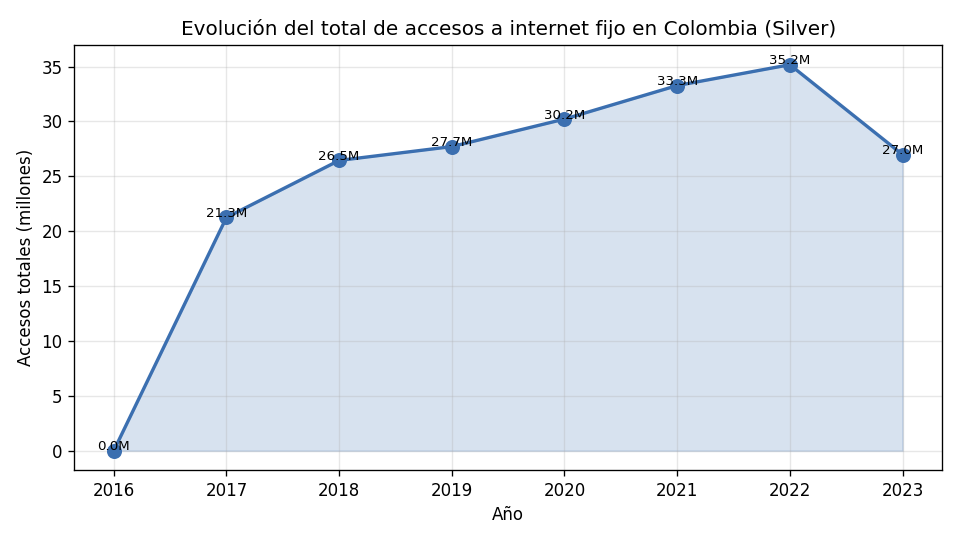
\includegraphics[width=0.9\textwidth]{figures/internet_evolucion_anual.png}
\caption{Evolución del total de accesos a internet fijo en Colombia (millones de accesos por año, tras filtros de calidad Silver).}
\end{figure}

La línea sube de manera sostenida, casi sin interrupciones, lo que refleja la masificación del servicio de internet fijo en Colombia durante la última década. La aceleración alrededor de 2020-2021 coincide con el período de confinamiento por la pandemia, momento en que la conectividad doméstica pasó de ser deseable a indispensable. Este patrón temporal es coherente con la literatura citada en la sección de entendimiento del negocio, donde se documenta el efecto post-pandemia sobre los hábitos digitales. Una observación operativa importante: los primeros años (2014-2015) tienen valores bastante inferiores que sugieren cobertura parcial del reporte, por lo que cualquier análisis longitudinal debe tomar en cuenta que la base no estaba completamente madura en sus inicios.

\textbf{La oferta tecnológica.} El cuadro de tecnologías muestra qué tipo de infraestructura sostiene la mayor parte del servicio.

\begin{figure}[H]
\centering
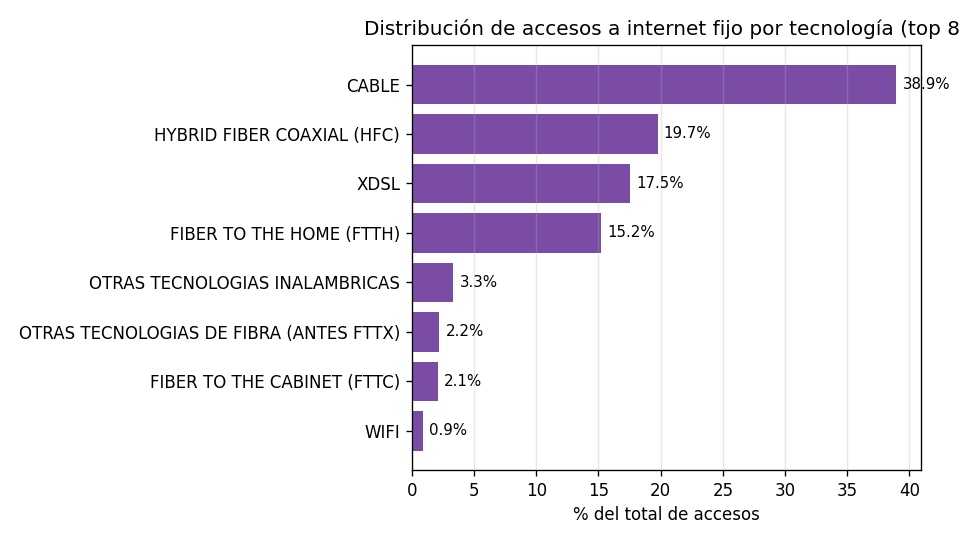
\includegraphics[width=0.9\textwidth]{figures/internet_top_tecnologias.png}
\caption{Distribución de accesos a internet fijo por tecnología utilizada (top 8 tecnologías).}
\end{figure}

La tabla revela una coexistencia interesante entre tecnologías tradicionales (Cable, HFC, XDSL) y la fibra óptica (FTTH), que ha ganado terreno aceleradamente en años recientes. Esta diversidad tecnológica es relevante para el análisis posterior porque la calidad del servicio varía sustancialmente entre tecnologías: la fibra ofrece velocidades muy superiores al XDSL tradicional, por ejemplo. Por eso, en el modelado posterior se conserva la variable de velocidad de bajada como feature, no solo el conteo de accesos.

\textbf{Calidad y duplicados.} El dataset presentó dos retos principales. Primero, los campos de velocidad llegan como texto con coma decimal (por ejemplo, \texttt{"8,00"}), un legado del locale es-CO que sin parseo dejaría todas las velocidades como nulos. Segundo, el dataset contiene una cantidad significativa de duplicados exactos (más de 82,000 grupos de duplicados que suman cerca de 173,000 filas), lo que de no corregirse sobreestimaría la cantidad de accesos en cualquier agregación. Ambos problemas se tratan formalmente en la sección de filtros y transformaciones.

\subsection{Personas Sisbén (DNP)}
El Sisbén es la fuente que aporta el contexto socioeconómico al proyecto. Sin esta base sería imposible entender en qué medida la pobreza estructural condiciona los resultados académicos. La tabla consolidada tiene 4,465,955 personas distribuidas en 1,099 municipios y 48 columnas, lo que en HDFS ocupa cerca de 937 MB. A diferencia de los demás datasets, el Sisbén trabaja a grano persona, lo que obligará posteriormente a un proceso de agregación para poder integrarlo con las otras fuentes a nivel municipal.

\textbf{La población que el Sisbén caracteriza.} La distribución por grupo (la clasificación oficial del programa) es la primera radiografía de la base.

\begin{figure}[H]
\centering
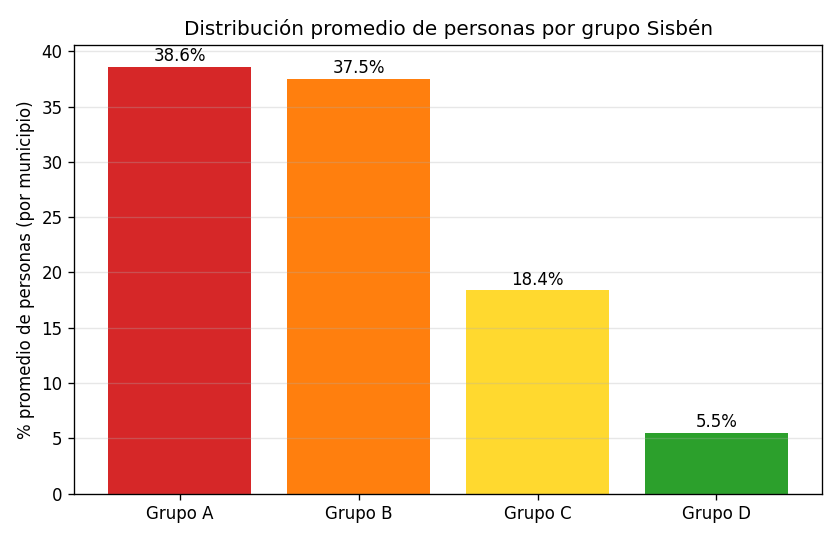
\includegraphics[width=0.75\textwidth]{figures/sisben_distribucion_grupos.png}
\caption{Distribución promedio de personas por grupo Sisbén a nivel municipio. Grupo A es la población más vulnerable; grupo D es la menos.}
\end{figure}

El gráfico confirma que el Sisbén concentra su registro en los grupos más vulnerables: en promedio, casi la mitad de las personas registradas en cualquier municipio pertenecen al grupo A (el de mayor privación), un 30\% al grupo B, un 16\% al grupo C y solo un 5\% al grupo D. Esto tiene sentido si se considera que el Sisbén es el instrumento de focalización de programas sociales del Estado: registra prioritariamente a quienes pueden ser beneficiarios. Para el proyecto esto implica que las variables derivadas del Sisbén (índice de privación, porcentaje en grupo A, etc.) son potentes señales de vulnerabilidad, pero deben interpretarse con cuidado al compararlas entre municipios cuya cobertura del registro Sisbén puede ser desigual.

\textbf{La conexión con el rendimiento académico.} Aunque la pregunta de cómo la pobreza incide en el puntaje Saber 11 se aborda formalmente en secciones posteriores, ya en exploración aparece una señal robusta cuando cruzamos las dos fuentes.

\begin{figure}[H]
\centering
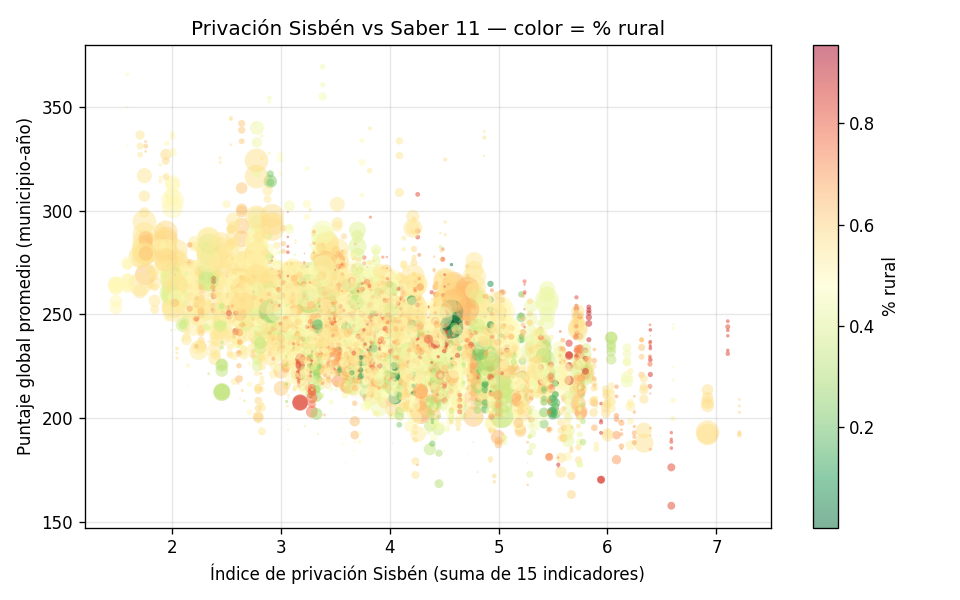
\includegraphics[width=0.95\textwidth]{figures/sisben_priv_vs_punt.png}
\caption{Índice de privación Sisbén vs puntaje global Saber 11 a nivel municipio-año. Tamaño del punto: número de estudiantes. Color: porcentaje rural del municipio (verde = urbano, rojo = rural).}
\end{figure}

La nube de puntos descendente es inconfundible: a mayor índice de privación (más privaciones promedio por persona), menor el puntaje promedio del municipio. El gradiente de color añade una segunda capa: los municipios más rurales (rojos) tienden a estar tanto en zonas de alta privación como en zonas de bajo puntaje, lo que sugiere que la geografía, la pobreza y el rendimiento académico son ejes que se mueven juntos. Esta observación es uno de los hallazgos centrales que el modelado posterior cuantifica con métricas formales.

\textbf{Calidad del dataset.} El Sisbén destaca por su completitud. Las variables clave de identificación (código de municipio, grupo, clasificación) no presentan nulos. Los 15 indicadores binarios de privación están bien tipificados y consistentes con la documentación oficial. La única decisión técnica importante fue la agregación de persona a municipio, que se realiza calculando promedios y porcentajes ponderados, transformando los 4.5 millones de personas en aproximadamente 1,099 filas municipales aptas para los joins multi-fuente.

\subsection{Educación MEN}
La fuente del Ministerio de Educación cierra el cuarteto. Su valor radica no en el volumen, sino en la riqueza temática: es la única que aporta indicadores estructurales del sistema educativo a nivel municipal y la única que ofrece la dimensión temporal completa del proyecto. La tabla consolidada tiene 15,707 registros y 41 columnas, cubriendo 1,124 municipios en 14 vigencias anuales entre 2011 y 2024.

\textbf{La evolución de la cobertura educativa.} El indicador principal del MEN es la cobertura neta. Su evolución por nivel educativo revela las dinámicas estructurales del sistema.

\begin{figure}[H]
\centering
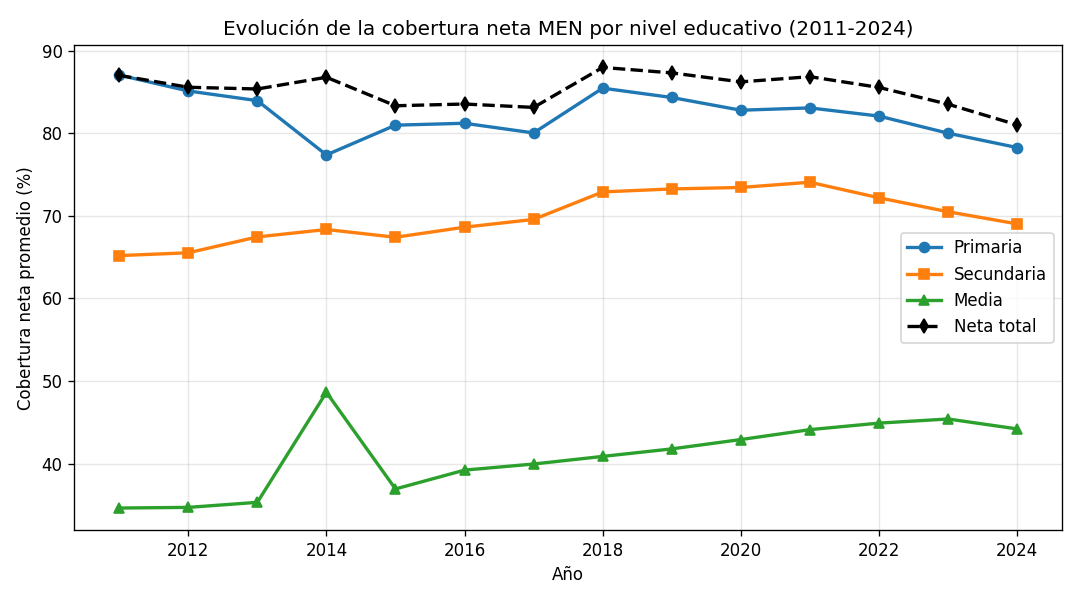
\includegraphics[width=0.95\textwidth]{figures/men_evolucion_cobertura.png}
\caption{Evolución de la cobertura neta promedio nacional por nivel educativo (2011-2024).}
\end{figure}

El gráfico muestra una historia compleja. La cobertura en primaria se mantiene relativamente alta a lo largo de toda la serie (entre 70\% y 80\%), confirmando que el problema del acceso inicial al sistema educativo está sustancialmente resuelto a nivel nacional. La cobertura en secundaria, en cambio, oscila entre el 60\% y el 70\%, dejando un margen importante de estudiantes que no completan ese tránsito. Pero el dato más llamativo es la cobertura en media: se ubica consistentemente alrededor del 40-45\%, menos de la mitad de la cobertura en primaria. Esta brecha progresiva entre niveles es un problema estructural reconocido del sistema educativo colombiano: muchos estudiantes ingresan al sistema pero se pierden en el camino antes de llegar a la educación media, que es justo el nivel en que se presenta la prueba Saber 11. Esta observación tiene una implicación directa para el proyecto: el dataset Saber 11 mide solo a quienes llegan, lo que invisibiliza una porción importante de la población joven del país.

\textbf{Calidad y particularidades.} La base presenta calidad alta en sus identificadores territoriales pero algunos retos en variables derivadas. Los nombres de las columnas vienen con acentos y caracteres especiales (\texttt{CÓDIGO\_MUNICIPIO}, \texttt{POBLACIÓN\_5\_16}), lo que rompe la selección por nombre en Spark y obliga a una normalización mediante slugify. Las variables porcentuales llegan como cadenas de texto con sufijo (\texttt{"56.11\%"}), lo que requiere parseo a doble. Adicionalmente, durante la ingesta se detectaron dos archivos del MEN con contenido byte-idéntico (verificado por hash MD5), lo que permitió eliminar uno sin pérdida de información y liberar espacio en el cluster. Todas estas decisiones técnicas se documentan en detalle en la sección de filtros y transformaciones del documento.

\subsection{Síntesis de la exploración}
La revisión de las cuatro fuentes deja varias conclusiones que orientan el resto del proyecto. Primero, las hipótesis del entendimiento del negocio se confirman cualitativamente: existe relación entre conectividad y rendimiento, existe brecha rural-urbana, existe correlación negativa entre pobreza multidimensional y puntaje, y existe heterogeneidad territorial fuerte en todas las dimensiones. Segundo, los principales problemas de calidad están identificados y son tratables con transformaciones estándar de Spark: nulos significativos en ICFES (37\% sin puntaje), duplicados en Internet Fijo, formatos de texto que requieren parseo en velocidades y porcentajes, nombres de columnas con caracteres especiales en MEN. Tercero, las cuatro fuentes comparten una clave común (el código DANE de municipio) que permite integrarlas, lo cual es el cimiento sobre el que se construye la vista minable Gold descrita más adelante.

Con esta base de entendimiento se procede a formalizar las preguntas de negocio que el proyecto se propone responder, las cuales se desarrollan en la siguiente subsección y se contestan formalmente en una sección posterior del documento.

\section{Planteamiento de preguntas de negocio}

Con base en la exploración inicial de las fuentes de datos, se plantean las siguientes preguntas de negocio para orientar las fases posteriores del análisis:

\begin{itemize}
    \item ¿Cuál es la relación entre el acceso a internet en el hogar y el desempeño académico de los estudiantes en las pruebas Saber 11 a nivel municipal?
    \item ¿Cómo varía el rendimiento en las pruebas Saber 11 entre zonas rurales y urbanas en función del nivel de conectividad digital de los municipios?
    \item ¿En qué medida la pobreza multidimensional incide en los resultados académicos, incluso en territorios con niveles similares de acceso a internet?
    \item ¿Qué diferencias en el desempeño académico se observan entre municipios con alta y baja penetración del servicio de internet?
    \item ¿Qué variables socioeconómicas presentan mayor capacidad explicativa del desempeño en Saber 11 en comparación con el acceso a internet?
    \item ¿Cuál es la relación entre la cobertura educativa (matrícula y asistencia) y el nivel de conectividad digital en los municipios analizados?
    \item ¿Cómo influye el acceso a computador en el hogar en los resultados obtenidos por los estudiantes en las diferentes áreas evaluadas en Saber 11?
    \item ¿Qué municipios presentan altos niveles de conectividad digital pero bajos resultados académicos, y qué patrones pueden identificarse en estos casos?
\end{itemize}
